 
\chapter{Logistic Regression for Binary Outcomes}
 \label{chapter::binary-logit}

Many applications have binary outcomes $y_i \in \{0, 1\}$. This chapter discusses statistical models of binary outcomes, focusing on the logistic regression.  


\section{Regression with binary outcomes}






\subsection{Linear probability model}

For simplicity, we can still use the linear model for a binary outcome. It is also called the linear probability model:
\[
y_{i}=x_{i}^{\T}\beta+\varepsilon_{i},\qquad E(\varepsilon_{i}\mid x_{i})=0
\]
because the conditional probability of $y_{i}$ given $x_{i}$ is
a linear function of $x_{i}$: 
\[
\pr(y_{i}=1\mid x_{i})=E(y_{i}\mid x_{i})=x_{i}^{\T}\beta.
\]
An advantage of this linear model is  that the interpretation of the coefficient remains the same as linear models for general outcomes:
$$
\frac{ \partial  \pr(y_{i}=1\mid x_{i})  }{  \partial x_{ij} } = \beta_j,
$$
that is, $\beta_j$ measures the partial impact of $x_{ij}$ on the probability of $y_i$. 


A minor technical issue is that the linear probability model implies heteroskedasticity because
$$
\var(y_i\mid x_i) = x_{i}^{\T}\beta (1-x_{i}^{\T}\beta).
$$
Therefore, we must use the EHW covariance based on OLS. We can also use FGLS to improve efficiency over OLS. 


A more severe problem with the linear probability model is its plausibility in general. We may not believe that a linear model is the correct model for a binary outcome because the probability $\pr(y_{i}=1\mid x_{i})$ on the left-hand side is bounded between zero and one, but the linear combination $x_{i}^{\T}\beta$ on the right-hand side can be unbounded for general covariates and coefficient. Nevertheless, the OLS decomposition $y_{i}=x_{i}^{\T}\beta+\varepsilon_{i}$
works for any $y_{i}\in\mathbb{R}$, so it is applicable for binary
$y_i$. Sometimes, practitioners feel that the linear model is not natural for binary outcomes because
the predicted value can be outside the range of $[0,1]$. Therefore,
it is more reasonable to build a model that automatically accommodates
the binary feature of the outcome. 


\subsection{General link functions}

A linear combination of general covariates may be outside the range
of $[0,1]$, but we can find a monotone transformation to force it
to lie within the interval $[0,1]$. This motivates us to consider the
following model:
\[
\pr(y_{i}=1\mid x_{i})=g(x_{i}^{\T}\beta),
\]
where $g(\cdot):\mathbb{R}\rightarrow[0,1]$ is a monotone function,
and its inverse is often called the link function. Mathematically,
the distribution function of any continuous random variable is a monotone function that maps from $\mathbb{R}$
to $[0,1]$. So we have infinitely many choices for $g(\cdot)$. Four
canonical choices ``logit'', ``probit'', ``cauchit'', and ``cloglog'' are below which are the standard options in \ri{R}: 

 
\begin{tabular}{|c|c|}
name & functional form\tabularnewline
\hline 
\hline 
logit & $g(z)=\frac{e^{z}}{1+e^{z}}$\tabularnewline
\hline 
probit & $g(z)=\Phi(z)$\tabularnewline
\hline 
cauchit & $g(z)=\frac{1}{\pi}\arctan(z)+\frac{1}{2}$\tabularnewline
\hline 
cloglog & $g(z)=1-\exp(-e^{z})$\tabularnewline
\end{tabular} 
 



The above $g(z)$'s correspond to different distribution functions. The $g(z)$ for the logit model\footnote{\citet{berkson1944application} was an early use of the logit model.}
is the distribution function of the standard logistic distribution
with density
\begin{equation}
g'(z)=\frac{e^{z}}{(1+e^{z})^{2}}=g(z)\left\{ 1-g(z)\right\} . \label{eq:densityoflogit}
\end{equation}
The $g(z)$ for the probit model\footnote{\citet{bliss1934method} was an early use of the probit model.} is the distribution function of a
standard Normal distribution. The $g(z)$ for the cauchit model is
the distribution function of the standard Cauchy distribution with
density
\[
g'(z)=\frac{1}{\pi(1+z^{2})} .
\]
The $g(z)$ for the cloglog model is the distribution function of the standard
log-Weilbull distribution with density
\[
g'(z)=\exp(z-e^{z}).
\]
I will give more motivations for the first three link functions in Section \ref{sec::binary-reg-latent} and for the fourth link function in Problem \ref{hw19::poisson-logistic}. 


\begin{figure}
\centering
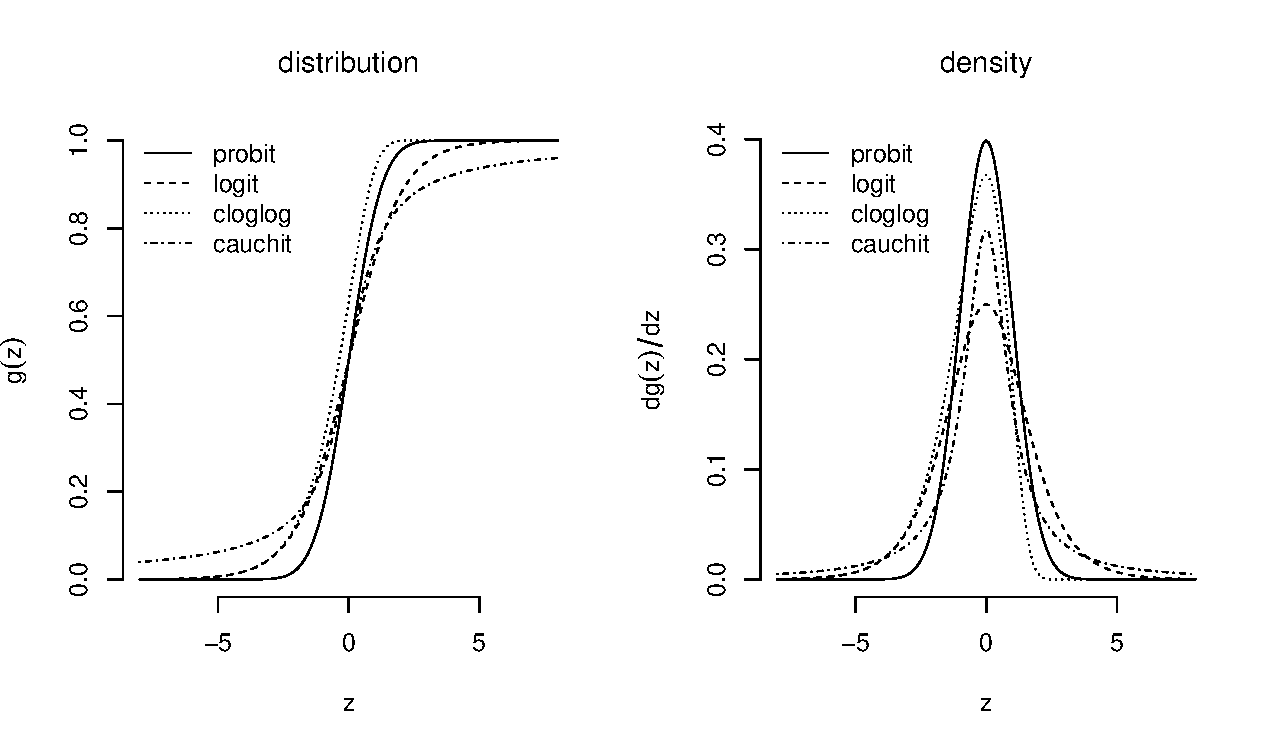
\includegraphics[width = \textwidth]{figures/binomiallinkfunctions.pdf}
\caption{Distributions and densities corresponding to the link functions}\label{fig::links-cdf=pdf}
\end{figure}

Figure \ref{fig::links-cdf=pdf} shows the distributions and densities of the corresponding link functions. The distribution functions are quite similar for all links, but the density for cloglog is asymmetric although all other three densities are symmetric. 



This chapter will focus on the logit model, and extensions to other models are conceptually straightforward. We can also write the logit model as
\begin{equation}
\pr(y_{i}=1\mid x_{i})\equiv\pi(x_{i},\beta)=\frac{e^{x_{i}^{\T}\beta}}{1+e^{x_{i}^{\T}\beta}},\label{eq:logit-parametric-model}
\end{equation}
for the conditional probability of $y_{i}$ 
given $x_{i}$, 
or, equivalently,
\[
\text{logit}\left\{ \pr(y_{i}=1\mid x_{i})\right\} \equiv\log\frac{\pr(y_{i}=1\mid x_{i})}{1-\pr(y_{i}=1\mid x_{i})}=x_{i}^{\T}\beta,
\]
for the log of the odds of $y_{i}$ 
given $x_{i}$, with the logit function
$$
\text{logit}(\pi) = \log \frac{ \pi }{1 - \pi}. 
$$
Because $y_{i}$ is a binary random variable, its
probability completely determines its distribution. So we can also
write the logit model as
\[
y_{i}\mid x_{i}\sim\text{Bernoulli}\left(\frac{e^{x_{i}^{\T}\beta}}{1+e^{x_{i}^{\T}\beta}}\right).
\]
Each coefficient $\beta_{j}$ measures the impact of $x_{ij}$ on the log odds of the outcome:
 $$
 \frac{ \partial  }{  \partial x_{ij} }  \text{logit} \{ \pr(y_{i}=1\mid   x_i ) \} = \beta_j .
 $$
Epidemiologists also call $\beta_{j}$ the
 conditional
log odds ratio because 
\begin{align*}
\beta_{j} & =\text{logit}\left\{ \pr(y_{i}=1\mid  \ldots,x_{ij}+1,\ldots )\right\} -\text{logit}\left\{ \pr(y_{i}=1\mid  \ldots,x_{ij},\ldots )\right\} \\
 & =\log\frac{\pr(y_{i}=1\mid  \ldots,x_{ij}+1 )}{1-\pr(y_{i}=1\mid  \ldots,x_{ij}+1 )} 
 - \log\frac{\pr(y_{i}=1\mid  \ldots,x_{ij},\ldots )}{1-\pr(y_{i}=1\mid  \ldots,x_{ij},\ldots )} \\
 &= \log \left\{
 \frac{\pr(y_{i}=1\mid \ldots,x_{ij}+1,\ldots )}{1-\pr(y_{i}=1\mid  \ldots,x_{ij}+1,\ldots )} 
 \Big/
\frac{\pr(y_{i}=1\mid  \ldots,x_{ij},\ldots )}{1-\pr(y_{i}=1\mid  \ldots,x_{ij},\ldots )} 
 \right\},
\end{align*}
that is, the change of the log odds of $y_{i}$ if we increase $x_{ij}$
by a unit holding other covariates unchanged. 
Qualitatively, if $\beta_j >0$, then larger values of $x_{ij}$ lead to larger probability of $y_i = 1$; if $\beta_j < 0$, then larger values of $x_{ij}$ lead to smaller probability of $y_i = 1$. 



\section{Maximum likelihood estimator of the logistic model}

Because we have specified a fully parametric model for $y_{i}$ given
$x_{i}$, we can estimate $\beta$ using the maximum likelihood. With
independent observations,   the likelihood function for
general binary outcomes is\footnote{The notation can be confusing because $\beta$ denotes both the true parameter and the dummy variable for the likelihood function.}
\begin{eqnarray*}
L(\beta) &=& 
\prod_{i=1}^{n} f(y_i\mid x_i) \\
&=& 
\prod_{i=1}^{n}   \left\{  \pi(x_{i},\beta) \text{ if } y_i = 1 \text{ or } 1-\pi(x_{i},\beta) \text{ if } y_i = 0  \right\} \\
&=&
\prod_{i=1}^{n}\left\{ \pi(x_{i},\beta)\right\} ^{y_{i}}\left\{ 1-\pi(x_{i},\beta)\right\} ^{1-y_{i}}.
\end{eqnarray*}
Under the logit form (\ref{eq:logit-parametric-model}), the likelihood function simplifies to
\begin{align*}
L(\beta) & =\prod_{i=1}^{n}\left\{ \frac{\pi(x_{i},\beta)}{1-\pi(x_{i},\beta)}\right\} ^{y_{i}}\left\{ 1-\pi(x_{i},\beta)\right\} \\
 & =\prod_{i=1}^{n}\left(e^{x_{i}^{\T}\beta}\right)^{y_{i}}\frac{1}{1+e^{x_{i}^{\T}\beta}}\\
 & =\prod_{i=1}^{n}\frac{e^{y_{i}x_{i}^{\T}\beta}}{1+e^{x_{i}^{\T}\beta}}.
\end{align*}
The log-likelihood function is
\[
\log L(\beta)=\sumn\left\{ y_{i}x_{i}^{\T}\beta-\log(1+e^{x_{i}^{\T}\beta})\right\} ,
\]
the score function is
\begin{align*}
\frac{\partial\log L(\beta)}{\partial\beta} & =\sumn\left(x_{i}y_{i}-\frac{x_{i}e^{x_{i}^{\T}\beta}}{1+e^{x_{i}^{\T}\beta}}\right)\\
 & =\sumn x_{i}\left(y_{i}-\frac{e^{x_{i}^{\T}\beta}}{1+e^{x_{i}^{\T}\beta}}\right)\\
 &= \sumn x_{i}\left\{  y_{i}-  g(x_{i}^{\T} \beta)  \right\} \\
 & =\sumn x_{i}\left\{ y_{i}-\pi(x_{i},\beta)\right\} ,
\end{align*}
and the Hessian matrix
\begin{align*}
\frac{\partial^{2}\log L(\beta)}{\partial\beta\partial\beta^{\T}} & =\left(\frac{\partial^{2}\log L(\beta)}{\partial\beta_{j}\partial\beta_{j'}}\right)_{1\leq j,j'\leq p}\\
 & =-\sumn x_{i}\frac{\partial g(x_{i}^{\T}\beta)}{\partial\beta^{\T}}\\
 & \stackrel{(\ref{eq:densityoflogit})}{=}-\sumn x_{i}x_{i}^{\T}g(x_{i}^{\T}\beta)\left\{ 1-g(x_{i}^{\T}\beta)\right\} \\
 & =-\sumn\pi(x_{i},\beta)\left\{ 1-\pi(x_{i},\beta)\right\} x_{i}x_{i}^{\T}.
\end{align*}
For any $\alpha \in \mathbb{R}^p$, we have
$$
\alpha^{\T}  \frac{\partial^{2}\log L(\beta)}{\partial\beta\partial\beta^{\T}} \alpha
=-\sumn\pi(x_{i},\beta)\left\{ 1-\pi(x_{i},\beta)\right\} (\alpha^{\T} x_{i} )^2 \leq 0
$$
so the Hessian matrix is negative semi-definite.
%\begin{eqnarray}
%\frac{\partial^{2}\log L(\beta)}{\partial\beta\partial\beta^{\T}}  \preceq 0, \label{eq::negativehessian}
%\end{eqnarray}
If it is negative
definite, then the likelihood function has a unique maximizer. 

The maximum likelihood estimate (MLE) must satisfy the following score or Normal equation:
\[
\sumn x_{i}\left\{ y_{i}-\pi(x_{i},\hat{\beta})\right\} =\sumn x_{i}\left(y_{i}-\frac{e^{x_{i}^{\T}\hat{\beta}}}{1+e^{x_{i}^{\T}\hat{\beta}}}\right)=0.
\]
If we view $\pi(x_{i},\hat{\beta})$ as the fitted probability
for $y_{i},$ then $y_{i}-\pi(x_{i},\hat{\beta})$ is the residual,
and the score equation is similar to that of OLS. Moreover, if $x_{i}$
contains $1$, then 
\[
\sumn\left\{ y_{i}-\pi(x_{i},\hat{\beta})\right\} =0 \Longrightarrow n^{-1}\sumn y_{i}=n^{-1}\sumn\pi(x_{i},\hat{\beta}),
\]
 that is the average of the outcomes equals the average of their fitted
values. 

However, the score equation is nonlinear, and in general, there is
no explicit formula for the MLE. We usually use Newton's method to
solve for the MLE based on the linearization of the score equation. Starting from the old value $\beta^{\text{old}}$, we can approximate the score equation by a linear equation:
\[
0=\frac{\partial\log L( \beta )}{\partial\beta}\cong\frac{\partial\log L(\beta^{\text{old}})}{\partial\beta}+\frac{\partial^{2}\log L(\beta^{\text{old}})}{\partial\beta\partial\beta^{\T}}(\beta-\beta^{\text{old}}),
\]
and then update
\[
\beta^{\text{new}}=\beta^{\text{old}}-\left\{ \frac{\partial^{2}\log L(\beta^{\text{old}})}{\partial\beta\partial\beta^{\T}}\right\} ^{-1}\frac{\partial\log L(\beta^{\text{old}})}{\partial\beta}.
\]
Using the matrix form, we can gain more insight from Newton's method.
Recall that 
$$
Y=\left(\begin{array}{c}
y_{1}\\
\vdots\\
y_{n}
\end{array}\right), \quad  X=\left(\begin{array}{c}
x_{1}^{\T}\\
\vdots\\
x_{n}^{\T}
\end{array}\right),
$$
and define 
$$
\Pi^{\text{old}}=\left(\begin{array}{c}
\pi(x_{1},\beta^{\text{old}})\\
\vdots\\
\pi(x_{n},\beta^{\text{old}})
\end{array}\right), \quad
 W^{\text{old}}=\text{diag}\left[\pi(x_{i},\beta^{\text{old}})\left\{ 1-\pi(x_{i},\beta^{\text{old}})\right\} \right]_{i=1}^{n}.
$$ 
Then 
\begin{align*}
\frac{\partial\log L(\beta^{\text{old}})}{\partial\beta} & =X^{\T}(Y  - \Pi^{\text{old}}),\\
\frac{\partial^{2}\log L(\beta^{\text{old}})}{\partial\beta\partial\beta^{\T}} & =-X^{\T}W^{\text{old}}X,
\end{align*}
and Newton's method simplifies to
\begin{align*}
\beta^{\text{new}} & =\beta^{\text{old}}+(X^{\T}W^{\text{old}}X)^{-1}X^{\T}(Y-\Pi^{\text{old}})\\
 & =(X^{\T}W^{\text{old}}X)^{-1}\left\{ X^{\T}W^{\text{old}}X\beta^{\text{old}}+X^{\T}(Y-\Pi^{\text{old}})\right\} \\
 & =(X^{\T}W^{\text{old}}X)^{-1}X^{\T}W^{\text{old}}Z^{\text{old}},
\end{align*}
where
\[
Z^{\text{old}}=X\beta^{\text{old}}+(W^{\text{old}})^{-1}(Y-\Pi^{\text{old}}).
\]
So we can obtain $\beta^{\text{new}}$ based on the WLS
fit of $Z^{\text{old}}$ on $X$ with weights $W^{\text{old}}$, the diagonal elements of which
are the conditional variances of the $y_{i}$'s given the $x_{i}$'s at $\beta^{\text{old}}$.
The \ri{glm} function in \ri{R} uses the Fisher scoring algorithm, which is
identical to Newton's method for the logit model\footnote{The Fisher scoring algorithm uses a slightly different approximation:
$$
0=\frac{\partial\log L( \beta )}{\partial\beta}\cong\frac{\partial\log L(\beta^{\text{old}})}{\partial\beta}
+  E\left\{ \frac{\partial^{2}\log L(\beta^{\text{old}})}{\partial\beta\partial\beta^{\T}}  \mid X \right\} (\beta-\beta^{\text{old}}) ,
$$ 
with the expected Fisher information instead of the observed Fisher information. For other link functions, the Fisher scoring algorithm is different from Newton's method. 
}. Sometimes, it is
also called the iteratively reweighted least squares algorithm. 



\section{Statistics with the logit model}





\subsection{Inference}

Based on the general theory of MLE, $\hat{\beta}$ is consistent for
$\beta$ and is asymptotically Normal. Approximately, we can conduct
statistical inference based on
\[
\hat{\beta}\asim \N\left\{ \beta,\left(-\frac{\partial^{2}\log L(\hat{\beta})}{\partial\beta\partial\beta^{\T}}\right)^{-1}\right\} 
=\N\left\{ \beta, (X^{\T}\hat{W}X)^{-1} \right\},
\]
where 
\[
\hat{W}=\text{diag}\left[\pi(x_{i},\hat{\beta})\left\{ 1-\pi(x_{i},\hat{\beta} )\right\} \right]_{i=1}^{n}.
\]
Based on this, the \ri{glm} function reports the point estimate, standard error, $z$-value, and $p$-value for each coordinate of $\beta$. It is almost identical to the output of the \ri{lm} function, except that the interpretation of the coefficient becomes the conditional log odds ratio. 



I use the data from \citet{hirano2000assessing} to illustrate logistic regression, where the main interest is the effect of the encouragement of receiving the flu shot via email on the binary indicator of flu-related hospitalization. We can fit a logistic regression using the \ri{glm} function in \ri{R} with \ri{family = binomial(link = logit)}. 

\begin{lstlisting}
> flu = read.table("fludata.txt", header = TRUE)
> flu = within(flu, rm(receive))
> assign.logit = glm(outcome ~ ., 
+                    family  = binomial(link = logit), 
+                    data    = flu)
> summary(assign.logit)

Call:
glm(formula = outcome ~ ., family = binomial(link = logit), data = flu)

Deviance Residuals: 
    Min       1Q   Median       3Q      Max  
-1.1957  -0.4566  -0.3821  -0.3048   2.6450  

Coefficients:
             Estimate Std. Error z value Pr(>|z|)    
(Intercept) -2.199815   0.408684  -5.383 7.34e-08 ***
assign      -0.197528   0.136235  -1.450  0.14709    
age         -0.007986   0.005569  -1.434  0.15154    
copd         0.337037   0.153939   2.189  0.02857 *  
dm           0.454342   0.143593   3.164  0.00156 ** 
heartd       0.676190   0.153384   4.408 1.04e-05 ***
race        -0.242949   0.143013  -1.699  0.08936 .  
renal        1.519505   0.365973   4.152 3.30e-05 ***
sex         -0.212095   0.144477  -1.468  0.14210    
liverd       0.098957   1.084644   0.091  0.92731    

(Dispersion parameter for binomial family taken to be 1)

    Null deviance: 1667.9  on 2860  degrees of freedom
Residual deviance: 1598.4  on 2851  degrees of freedom
AIC: 1618.4

Number of Fisher Scoring iterations: 5
\end{lstlisting}



Three subtle issues arise in the above code. First, \ri{flu = within(flu, rm(receive))} drops \ri{receive}, which is the indicator of whether a patient received the flu shot or not. The reason is that  \ri{assign} is randomly assigned but \ri{receive} is subject to selection bias, that is, patients receiving the flu shot can be quite different from patients not receiving the flu shot.



Second, the \ri{Null deviance} and \ri{Residual deviance} are defined as 
$
- 2 \log L(\tilde{\beta})
$
and
$
- 2 \log L(\hat{\beta}),
$
 respectively, where $\tilde{\beta}$ is the MLE assuming that all coefficients except the intercept are zero, and $\hat{\beta}$ is the MLE without any restrictions. They are not of independent interest, but their difference is: Wilks' theorem ensures that
 $$
 \{ - 2 \log L(\tilde{\beta}) \}  - \{- 2 \log L(\hat{\beta})\}
 =2 \log \frac{ L(\hat{\beta})  }{ L(\tilde{\beta}) } \asim \chi_{p-1}^2.
 $$
So we can test whether the coefficients of the covariates are all zero, which is analogous to the joint $F$ test in linear models. 

\begin{lstlisting}
> pchisq(assign.logit$null.deviance - assign.logit$deviance,
+        df = assign.logit$df.null - assign.logit$df.residual,
+        lower.tail = FALSE)
[1] 1.912952e-11
\end{lstlisting}


Third, the AIC is defined as $- 2 \log L(\hat{\beta}) + 2p$, where $p$ is the number of parameters in the logit model. This is also the general formula of AIC for other parametric models. 


\subsection{Prediction}

The logit model is often used for prediction or classification since the outcome is binary. With the MLE $\hat{\beta}$, we can predict the probability of being one as $\hat{\pi}_{n+1}  =  g(x_{n+1} ^{\T} \hat{\beta})$ for a unit with covariate value $x_{n+1} $, and we can easily dichotomize the fitted probability to predict the outcome itself by $\hat{y}_{n+1}  =  1(\hat{\pi}_{n+1}  \geq c)$, for example, with $c=0.5$. 


We can even quantify the uncertainty in the fitted probability based on a linear approximation (i.e., the delta method). Based on
\begin{eqnarray*}
\hat{\pi}_{n+1}   &=&  g(x_{n+1} ^{\T} \hat{\beta}) \\
&\cong&   g(x_{n+1} ^{\T} \beta) +  g'(x_{n+1} ^{\T}  \beta) x_{n+1} ^{\T} (\hat{\beta} - \beta) \\
&=&  g(x_{n+1} ^{\T} \beta) +  g(x_{n+1} ^{\T}  \beta )  \{1-g(x_{n+1} ^{\T}  \beta ) \} x_{n+1} ^{\T} (\hat{\beta} - \beta),
\end{eqnarray*}
we can approximate the asymptotic variance of $\hat{\pi}_{n+1}  $ by
$$
 [ g(x_{n+1} ^{\T}  \beta )  \{1-g(x_{n+1} ^{\T}  \beta ) \}  ]^2 x_{n+1} ^{\T}  (X^{\T}\hat{W}X)^{-1} x_{n+1} . 
$$


We can use the \ri{predict} function in \ri{R} to calculate the predicted values based on a \ri{glm} object in the same way as the linear model. If we specify \ri{type="response"}, then we obtain the fitted probabilities; if we specify \ri{se.fit = TRUE}, then we also obtain the standard errors of the fitted probabilities. In the following, I predict the probabilities of flu-related hospitalization if a patient receives the email encouragement or not, fixing other covariates at their empirical means. 


\begin{lstlisting}
> emp.mean = apply(flu, 2, mean)
> data.ave = rbind(emp.mean, emp.mean)
> data.ave[1, 1] = 1
> data.ave[2, 1] = 0
> data.ave = data.frame(data.ave)
> predict(assign.logit, newdata = data.ave,
+         type = "response", se.fit = TRUE)
$fit
  emp.mean emp.mean.1 
0.06981828 0.08378818 

$se.fit
   emp.mean  emp.mean.1 
0.006689665 0.007526307 
\end{lstlisting}



\section{More on interpretations of the coefficients}
%\subsection{Average partial effects}

Many practitioners find the coefficients in the logit model difficult to interpret. Another measure of the impact of the covariate on the outcome is the average marginal effect or average partial effect. For a continuous covariate $x_{ij}$, the average marginal effect is defined as 
\begin{eqnarray*}
\textsc{ame}_j 
&=& 
n^{-1}\sumn\frac{\partial\pr(y_{i}=1\mid x_{i})}{\partial x_{ij}} \\
&=& 
n^{-1}\sumn g'(x_{i}^{\T}\beta)\beta_{j},
\end{eqnarray*}
which reduces to the following form for the logit model
\[
\textsc{ame}_j = 
%n^{-1}\sumn\frac{\partial\pr(y_{i}=1\mid x_{i})}{\partial x_{ij}}=
\beta_{j}\times n^{-1}\sumn\pi(x_{i},\beta)\left\{ 1-\pi(x_{i},\beta)\right\} .
\]
For a binary covariate $x_{ij}$, the average marginal effect is defined as 
$$
\textsc{ame}_j = 
n^{-1}\sumn  \{  \pr(y_{i}=1\mid  \ldots, x_{ij}=1, \ldots) - \pr(y_{i}=1\mid  \ldots, x_{ij}=0, \ldots )  \} 
$$
The \ri{margins} function in the \ri{margins} package can compute the average marginal effects and the corresponding standard errors. In particular, the average marginal effect of \ri{assign} is not significant as shown below. The \ri{R} code in this section is in \ri{code19.3.R}. 


\begin{lstlisting}
> library("margins")
> ape = margins(assign.logit)
> summary(ape)
 factor     AME     SE       z      p   lower  upper
    age -0.0006 0.0004 -1.4322 0.1521 -0.0014 0.0002
 assign -0.0150 0.0103 -1.4480 0.1476 -0.0352 0.0053
   copd  0.0255 0.0117  2.1830 0.0290  0.0026 0.0485
     dm  0.0344 0.0109  3.1465 0.0017  0.0130 0.0559
 heartd  0.0512 0.0118  4.3441 0.0000  0.0281 0.0743
 liverd  0.0075 0.0822  0.0912 0.9273 -0.1536 0.1686
   race -0.0184 0.0109 -1.6958 0.0899 -0.0397 0.0029
  renal  0.1151 0.0278  4.1461 0.0000  0.0607 0.1696
    sex -0.0161 0.0110 -1.4660 0.1426 -0.0376 0.0054
\end{lstlisting}    

  
 
%\subsection{Difficulty of interpreting interaction}
The interaction term is much more complicated. Contradictory suggestions are given across fields. 
Consider
the following model
\[
\pr(y_{i}=1\mid x_{i1},x_{i2})=g(\beta_{0}+\beta_{1}x_{i1}+\beta_{2}x_{i2}+\beta_{12}x_{i1}x_{i2}).
\]
If the link is logit, then epidemiologists interpret $e^{\beta_{12}}$ as the interaction between $x_{i1}$ and $x_{i2}$ on the odds ratio scale. Consider a simple case with binary $x_{i1}$ and $x_{i2}$. Given $x_{i2} = 1$, the odds ratio of $x_{i1}$ on $y_i$ equals $e^{\beta_1 + \beta_{12}}$; given $x_{i2} = 0$, the odds ratio of $x_{i1}$ on $y_i$ equals $e^{\beta_1}$. Therefore, the ratio of the two odds ratio equals $e^{\beta_{12}}$.  When we measure effects on the odds ratio scale, the logistic model is a natural choice. The interaction term in the logistic model indeed measures the interaction of $x_{i1}$ and $x_{i2}$. 

\citet{ai2003interaction} gave a different suggestion. 
Define $z_i = \beta_{0}+\beta_{1}x_{i1}+\beta_{2}x_{i2}+\beta_{12}x_{i1}x_{i2}.$
We have two ways to define the interaction effect: first,
\[
n^{-1}\sumn\frac{\partial\pr(y_{i}=1\mid x_{i1},x_{i2})}{\partial(x_{i1}x_{i2})}
=n^{-1}\sumn g'(  z_i )\beta_{12}.
\]
second,
\begin{align*}
& n^{-1}\sumn\frac{\partial^{2}\pr(y_{i}=1\mid x_{i1},x_{i2})}{\partial x_{i1}\partial x_{i2}} \\
& =n^{-1}\sumn\frac{\partial}{\partial x_{i2}}\left\{ \frac{\partial\pr(y_{i}=1\mid x_{i1},x_{i2})}{\partial x_{i1}}\right\} \\
 & =n^{-1}\sumn\frac{\partial}{\partial x_{i2}}\left\{ g'(z_i)(\beta_{1}+\beta_{12}x_{i2})\right\} \\
 & =n^{-1}\sumn\left\{ g''( z_i )(\beta_{2}+\beta_{12}x_{i1})(\beta_{1}+\beta_{12}x_{i2})+g'(z_i)\beta_{12}\right\} ;
\end{align*}
Although the first one is more straightforward based on the definition of the average partial effect, the second one is more reasonable based on the natural definition of interaction based on the mixed derivative.  
Note that even if $\beta_{12} = 0$, the second definition of interaction 
does not necessarily equal 0 since
\begin{align*}
 n^{-1}\sumn\frac{\partial^{2}\pr(y_{i}=1\mid x_{i1},x_{i2})}{\partial x_{i1}\partial x_{i2}}  
 =n^{-1}\sumn   g''( z_i ) \beta_{1}  \beta_{2} . 
\end{align*}
 This is due to the nonlinearity of the link function. 
The second definition quantifies interaction based on the probability itself while the parameters in the logistic model measure the odds ratio. This combination of model and parameter does not seem a natural choice. 



\section{Does the link function matter?}

First, I generate data from a simple one-dimensional logistic model.

 
\begin{lstlisting}
> n  = 100
> x  = rnorm(n, 0, 3)
> prob = 1/(1 + exp(-1 + x))
> y  = rbinom(n, 1, prob)
\end{lstlisting}


Then I fit the data with the linear probability model and binary models with four link functions. 
\begin{lstlisting}
> lpmfit    = lm(y ~ x)
> probitfit = glm(y ~ x, family = binomial(link = "probit"))
Warning message:
glm.fit: fitted probabilities numerically 0 or 1 occurred 
> logitfit  = glm(y ~ x, family = binomial(link = "logit"))
> cloglogfit= glm(y ~ x, family = binomial(link = "cloglog"))
Warning message:
glm.fit: fitted probabilities numerically 0 or 1 occurred 
> cauchitfit= glm(y ~ x, family = binomial(link = "cauchit"))
\end{lstlisting}


 
The coefficients are quite different because the coefficients measure the association between $x$ and $y$ on difference scales. These parameters are not directly comparable.  
\begin{lstlisting}
> betacoef = c(lpmfit$coef[2], 
+              probitfit$coef[2], 
+              logitfit$coef[2], 
+              cloglogfit$coef[2], 
+              cauchitfit$coef[2])
> names(betacoef) = c("lpm", "probit", "logit", "cloglog", "cauchit")
> round(betacoef, 2)
    lpm  probit   logit cloglog cauchit 
  -0.10   -0.83   -1.47   -1.07   -2.09
\end{lstlisting}


However, if we care only about the prediction, then these five models give very similar results. 

\begin{lstlisting}
> table(y, lpmfit$fitted.values>0.5)
   
y   FALSE TRUE
  0    31    9
  1     5   55
> table(y, probitfit$fitted.values>0.5)
   
y   FALSE TRUE
  0    31    9
  1     5   55
> table(y, logitfit$fitted.values>0.5)
   
y   FALSE TRUE
  0    31    9
  1     5   55
> table(y, cloglogfit$fitted.values>0.5)
   
y   FALSE TRUE
  0    34    6
  1     7   53
> table(y, cauchitfit$fitted.values>0.5)
   
y   FALSE TRUE
  0    34    6
  1     7   53
  \end{lstlisting}
  
 
  
Figure \ref{fig::compare-links} shows the fitted probabilities versus the true probabilities $\pr(y_i =1\mid x_i)$. The patterns are quite similar although the linear probability model can give fitted probabilities outside $[0,1]$. When we use the cutoff point $0.5$ to predict the binary outcome, the problem of the linear probability model becomes rather minor. 


\begin{figure}
\centering
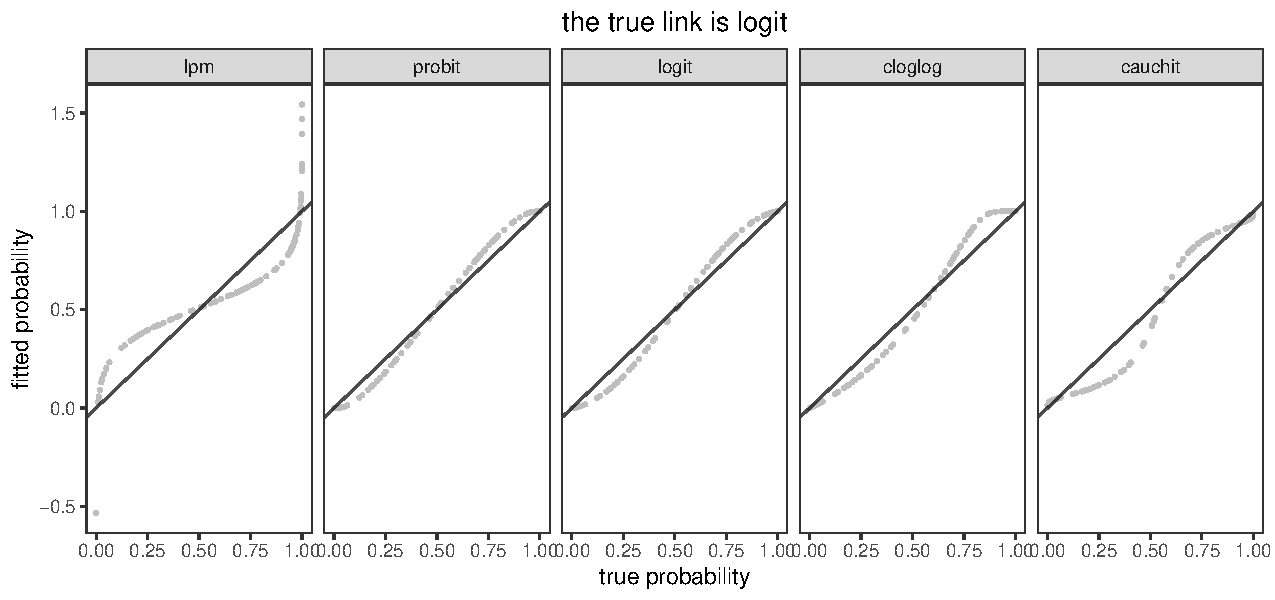
\includegraphics[width = \textwidth]{figures/fittedprobabilities.pdf}
\caption{Comparing the fitted probabilities from different link functions}\label{fig::compare-links}
\end{figure}



An interesting fact is that the coefficients from the logit model approximately equal those from the probit model multiplied by 1.7, a constant that minimizes $\max_y | g_{\text{logit}}(by) - g_{\text{probit}}(y) |$. We can easily compute this constant numerically:
\begin{lstlisting}
> d.logit.probit = function(b){
+   x = seq(-20, 20, 0.00001)
+   max(abs(plogis(b*x) - pnorm(x)))
+ }
> 
> optimize(d.logit.probit, c(-10, 10))
$minimum
[1] 1.701743

$objective
[1] 0.009457425
\end{lstlisting} 
Based on the above calculation, the maximum difference is approximately 0.009. Therefore, the logit and probit link functions are extremely close up to the scaling factor 1.7. However, $\min_b \max_y | g_{\text{logit}}(by) - g_{ * }(y) |$ is much larger for the link functions of cauchit and cloglog. 




\section{Extensions of the logistic regression}

\subsection{Penalized logistic regression}


Similar to the high dimensional linear model, we can also extend the logit model to a penalized version. Since the objective function for the original logit model is the log-likelihood, we can minimize the following penalized log-likelihood function: 
\[
\arg\min_{\beta_0,\beta_1, \ldots, \beta_p}-\frac{1}{n}\sumn \ell_i(\beta )   +\lambda\sum_{j=1}^{p} \{  \alpha \beta_j^2 + (1-\alpha)  |\beta_{j}| \} ,
\]
where 
$$
\ell_i(\beta) = y_{i}(\beta_{0}+\beta_{1}x_{i1}+\cdots+\beta_{p}x_{ip})-\log(1+e^{\beta_{0}+\beta_{1}x_{i1}+\cdots+\beta_{p}x_{ip}})
$$ 
is the log-likelihood function. When $\alpha = 1$, it gives the ridge analog of the logistic regression; when $\alpha = 0$, it gives the lasso analog; when $\alpha \in (0,1)$, it gives the elastic net analog. 
The \ri{R} package \ri{glmpath} uses the coordinate descent algorithm based on a quadratic
approximation of the log-likelihood function. We can select the tuning parameter $\lambda$ based on cross-validation. 

\subsection{Case-control study}\label{sec::case-control-study}


A nice property of the logit model is that it works not only for  the cohort study with data from conditional distribution $y_i\mid x_i$ but also for the case-control study with data from the conditional distribution $x_i\mid y_i$. The former is a prospective study while the latter is a retrospective study. Below, I will explain the basic idea in \citet{prentice1979logistic}. 


Assume that $(x_{i},y_{i},s_{i})$ IID with 
\begin{eqnarray}
\label{eq::cc=1}
\pr(y_i = 1\mid x_i) =  \frac{e^{\beta_{0}+x_{i}^{\T}\beta}}{1+e^{\beta_{0}+x_{i}^{\T}\beta}} 
\end{eqnarray}
and
\begin{eqnarray}
\label{eq::cc=2}
\pr(s_{i}=1\mid x_{i},y_{i})=\pr(s_{i}=1\mid y_{i})=\begin{cases}
p_{1}, & \text{if }y_{i}=1,\\
p_{0}, & \text{if }y_{i}=0.
\end{cases}
\end{eqnarray}
But we only have data with $s_{i}=1$ with $p_{1}$ and $p_{0}$ often
unknown. Fortunately, conditioning on $s_{i}=1$, we have the following result. 

\begin{theorem}
\label{thm::case-control}
Under \eqref{eq::cc=1} and \eqref{eq::cc=2}, we have 
$$
\pr(y_{i}  =1\mid x_{i},s_{i}=1)
= \frac{e^{\delta+\beta_{0}+x_{i}^{\T}\beta}}{1+e^{\delta+\beta_{0}+x_{i}^{\T}\beta}}, 
$$
where $\delta=\log(p_{1}/p_{0})$. 
\end{theorem}

\begin{myproof}{Theorem}{\ref{thm::case-control}}
We have 
\begin{align*}
&\pr(y_{i}  =1\mid x_{i},s_{i}=1)\\
 & =\frac{\pr(y_{i}=1\mid x_{i})\pr(s_{i}=1\mid x_{i},y_{i}=1)}{\pr(y_{i}=1\mid x_{i})\pr(s_{i}=1\mid x_{i},y_{i}=1)+\pr(y_{i}=0\mid x_{i})\pr(s_{i}=1\mid x_{i},y_{i}=0)}
 \end{align*}
 by Bayes' formula. Under the logit model, we have
 \begin{align*}
\pr(y_{i}  =1\mid x_{i},s_{i}=1)
 & =\frac{\frac{e^{\beta_{0}+x_{i}^{\T}\beta}}{1+e^{\beta_{0}+x_{i}^{\T}\beta}}p_{1}}{\frac{e^{\beta_{0}+x_{i}^{\T}\beta}}{1+e^{\beta_{0}+x_{i}^{\T}\beta}}p_{1}+\frac{1}{1+e^{\beta_{0}+x_{i}^{\T}\beta}}p_{0}}\\
 & =\frac{e^{\beta_{0}+x_{i}^{\T}\beta}p_{1}}{e^{\beta_{0}+x_{i}^{\T}\beta}p_{1}+p_{0}}\\
 & =\frac{e^{\beta_{0}+x_{i}^{\T}\beta}p_{1}/p_{0}}{e^{\beta_{0}+x_{i}^{\T}\beta}p_{1}/p_{0}+1}\\
 & =\frac{e^{\delta+\beta_{0}+x_{i}^{\T}\beta}}{1+e^{\delta+\beta_{0}+x_{i}^{\T}\beta}} . 
\end{align*}
\end{myproof}

Theorem \ref{thm::case-control} ensures that conditioning on $s_{i}=1$,
the model of $y_{i}$ given $x_{i}$ is still logit with the intercept
changing from $\beta_{0}$ to $\beta_{0}+\log(p_{1}/p_{0})$. Although
we cannot consistently estimate the intercept without knowing $(p_{1},p_{0})$,
we can still estimate all the slopes. \citet{kagan2001note} showed that the logistic link is the only one that enjoys this property. 


\citet{samarani2019activating} hypothesized that variation in the inherited activating Killer-cell Immunoglobulin-like Receptor genes in humans is associated with their innate susceptibility/resistance to developing Crohn's disease. They used a case-control study from three cities (Manitoba,  Montreal, and Ottawa) in Canada to investigate the potential association. 
 
\begin{lstlisting}
> dat  = read.csv("samarani.csv")
> pool.glm = glm(case_comb ~ ds1 + ds2 + ds3 + ds4_a + 
+                  ds4_b + ds5 + ds1_3 + center,
+                family = binomial(link = logit),
+                data = dat)
> summary(pool.glm)

Call:
glm(formula = case_comb ~ ds1 + ds2 + ds3 + ds4_a + ds4_b + ds5 + 
    ds1_3 + center, family = binomial(link = logit), data = dat)

Deviance Residuals: 
    Min       1Q   Median       3Q      Max  
-1.9982  -0.9274  -0.5291   1.0113   2.2289  

Coefficients:
               Estimate Std. Error z value Pr(>|z|)    
(Intercept)    -2.39681    0.21768 -11.011  < 2e-16 ***
ds1             0.55945    0.14437   3.875 0.000107 ***
ds2             0.42531    0.14758   2.882 0.003954 ** 
ds3             0.81377    0.14503   5.611 2.01e-08 ***
ds4_a           0.30270    0.30679   0.987 0.323802    
ds4_b           0.29199    0.17726   1.647 0.099511 .  
ds5             0.92049    0.14852   6.198 5.72e-10 ***
ds1_3           0.49982    0.14706   3.399 0.000677 ***
centerMontreal -0.05816    0.15889  -0.366 0.714316    
centerOttawa    0.14164    0.20251   0.699 0.484292    

(Dispersion parameter for binomial family taken to be 1)

    Null deviance: 1403.7  on 1020  degrees of freedom
Residual deviance: 1192.0  on 1011  degrees of freedom
AIC: 1212

Number of Fisher Scoring iterations: 3
\end{lstlisting}

 

\section{Other model formulations}

\subsection{Latent linear model}\label{sec::binary-reg-latent}

Let $y_{i}=1(y_{i}^{*}\geq0)$ where

\[
y_{i}^{*}=x_{i}^{\T}\beta + \varepsilon_{i}
\]
and $ - \varepsilon_{i}$ has distribution function $g(\cdot)$ and is
independent of $x_{i}$. From this latent linear model, we can verify
that 
\begin{align*}
\pr(y_{i}  =1\mid x_{i}) &=\pr(y_{i}^{*}\geq0\mid x_{i})\\
 & =\pr(x_{i}^{\T}\beta + \varepsilon_{i}\geq0\mid x_{i})\\
 & =\pr( - \varepsilon_{i}\leq x_{i}^{\T}\beta\mid x_{i})\\
 & =g(x_{i}^{\T}\beta).
\end{align*}
So the $g(\cdot)$ function can be interpreted as the distribution
function of the error term in the latent linear model. 


This latent variable formulation provides another way to interpret the coefficients in the models for binary data. It is a powerful way to generate models for more complex data. We will see another example in the next chapter. 




\subsection{Inverse model}\label{subsec:Inverse-model-gaussian-mixture}

Assume that 
\begin{eqnarray}
y_{i}\sim\text{Bernoulli}(q),
\label{eq::y-marginal}
\end{eqnarray}
and
\begin{eqnarray}
x_{i}\mid y_{i}=1\sim\N(\mu_{1},\Sigma),\quad x_{i}\mid y_{i}=0\sim\N(\mu_{0},\Sigma),
\label{eq::xgiveny}
\end{eqnarray} 
where $x_i$ does not contain $1$.
This is called the linear discriminant model. 
We can verify that $y_{i}\mid x_{i}$ follows a logit model as shown in the theorem below.  


\begin{theorem}
\label{thm::inverse-logit}
Under \eqref{eq::y-marginal} and \eqref{eq::xgiveny}, we have
$$
\textup{logit}\{  \pr(y_i =1\mid x_i) \} = \alpha + x_i^{\T} \beta, 
$$
where
\begin{eqnarray}
\label{eq::alpha-beta-lda}
\alpha = \log\frac{q}{1-q}-\frac{1}{2}\left(\mu_{1}^{\T}\Sigma^{-1}\mu_{1}-\mu_{0}^{\T}\Sigma^{-1}\mu_{0}\right)  ,\quad
\beta = \Sigma^{-1}\left(\mu_{1}-\mu_{0}\right) . 
\end{eqnarray}
\end{theorem}

\begin{myproof}{Theorem}{\ref{thm::inverse-logit}}
Using Bayes' formula, we have
\begin{align*}
\pr(y_{i}  =1\mid x_{i}) &=\frac{\pr(y_{i}=1,x_{i})}{\pr(x_{i})}\\
 & =\frac{\pr(y_{i}=1)\pr(x_{i}\mid y_{i}=1)}{\pr(y_{i}=1)\pr(x_{i}\mid y_{i}=1)+\pr(y_{i}=0)\pr(x_{i}\mid y_{i}=0)}\\
 &= \frac{ e^\Delta}{1+ e^\Delta},
% & =\frac{q\left\{ 2\pi\text{det}(\Sigma)\right\} ^{-p/2}\exp\left\{ -(x_{i}-\mu_{1})^{\T}\Sigma^{-1}(x_{i}-\mu_{1})/2\right\} }{q\left\{ 2\pi\text{det}(\Sigma)\right\} ^{-p/2}\exp\left\{ -(x_{i}-\mu_{1})^{\T}\Sigma^{-1}(x_{i}-\mu_{1})/2\right\} +(1-q)\left\{ 2\pi\text{det}(\Sigma)\right\} ^{-p/2}\exp\left\{ -(x_{i}-\mu_{0})^{\T}\Sigma^{-1}(x_{i}-\mu_{0})/2\right\} }\\
% & =\frac{q\exp\left\{ -(x_{i}-\mu_{1})^{\T}\Sigma^{-1}(x_{i}-\mu_{1})/2\right\} }{q\exp\left\{ -(x_{i}-\mu_{1})^{\T}\Sigma^{-1}(x_{i}-\mu_{1})/2\right\} +(1-q)\exp\left\{ -(x_{i}-\mu_{0})^{\T}\Sigma^{-1}(x_{i}-\mu_{0})/2\right\} }\\
% & =\frac{q\exp\left\{ -(x_{i}-\mu_{1})^{\T}\Sigma^{-1}(x_{i}-\mu_{1})/2\right\} }{q\exp\left\{ -(x_{i}-\mu_{1})^{\T}\Sigma^{-1}(x_{i}-\mu_{1})/2\right\} +(1-q)\exp\left\{ -(x_{i}-\mu_{0})^{\T}\Sigma^{-1}(x_{i}-\mu_{0})/2\right\} }.
\end{align*}
%
%Because 
%\[
%\exp\left\{ -(x_{i}-\mu)^{\T}\Sigma^{-1}(x_{i}-\mu)/2\right\} =\exp\left\{ -\left(x_{i}^{\T}\Sigma^{-1}x_{i}-2x_{i}^{\T}\Sigma^{-1}\mu+\mu^{\T}\Sigma^{-1}\mu\right)/2\right\} ,
%\]
%we have
%\begin{align*}
%\pr(y_{i} & =1\mid x_{i})=\frac{q\exp\left\{ -\left(-2x_{i}^{\T}\Sigma^{-1}\mu_{1}+\mu_{1}^{\T}\Sigma^{-1}\mu_{1}\right)/2\right\} }{q\exp\left\{ -\left(-2x_{i}^{\T}\Sigma^{-1}\mu_{1}+\mu_{1}^{\T}\Sigma^{-1}\mu_{1}\right)/2\right\} +(1-q)\exp\left\{ -\left(-2x_{i}^{\T}\Sigma^{-1}\mu_{0}+\mu_{0}^{\T}\Sigma^{-1}\mu_{0}\right)/2\right\} }\\
% & =\frac{\Delta}{1+\Delta},
%\end{align*}
where
\begin{align*}
\Delta 
&= \log  \frac{\pr(y_{i}=1)\pr(x_{i}\mid y_{i}=1)}{ \pr(y_{i}=0)\pr(x_{i}\mid y_{i}=0) } \\
&=\log \frac{q\left\{ (2\pi)^p \text{det}(\Sigma)\right\} ^{-1/2}\exp\left\{ -(x_{i}-\mu_{1})^{\T}\Sigma^{-1}(x_{i}-\mu_{1})/2\right\}}
{  (1-q)\left\{ (2\pi)^p \text{det}(\Sigma)\right\} ^{-1/2}\exp\left\{ -(x_{i}-\mu_{0})^{\T}\Sigma^{-1}(x_{i}-\mu_{0})/2\right\} }\\
&=\log \frac{q\exp\left\{ -(x_{i}-\mu_{1})^{\T}\Sigma^{-1}(x_{i}-\mu_{1})/2\right\}}
{  (1-q) \exp\left\{ -(x_{i}-\mu_{0})^{\T}\Sigma^{-1}(x_{i}-\mu_{0})/2\right\}  }\\
& =\log\frac{q\exp\left\{ -\left(-2x_{i}^{\T}\Sigma^{-1}\mu_{1}+\mu_{1}^{\T}\Sigma^{-1}\mu_{1}\right)/2\right\} }{(1-q)\exp\left\{ -\left(-2x_{i}^{\T}\Sigma^{-1}\mu_{0}+\mu_{0}^{\T}\Sigma^{-1}\mu_{0}\right)/2\right\} }\\
 & = \log\frac{q}{1-q}-\frac{1}{2}\left(\mu_{1}^{\T}\Sigma^{-1}\mu_{1}-\mu_{0}^{\T}\Sigma^{-1}\mu_{0}\right)+x_{i}^{\T}\Sigma^{-1}\left(\mu_{1}-\mu_{0}\right) . 
\end{align*}
So $y_{i}\mid x_{i}$ follows a logistic model with
$\alpha$ and $\beta$ given in \eqref{eq::alpha-beta-lda}. 
\end{myproof}


We can easily obtain the moment estimators for the unknown parameters under \eqref{eq::y-marginal} and \eqref{eq::xgiveny}. Let $n_1 = \sumn y_i$ and $n_0 = n-n_1$. The moment estimator for $q$ is 
$
\hat{q} = n_1/n,
$
the sample mean of the $y_i$'s. The moment estimators for $\mu_1$ and $\mu_0$ are
$$
\hat{\mu}_1 = n_1^{-1} \sumn  y_i x_i,\quad \hat{\mu}_0 = n_0^{-1} \sumn (1-y_i) x_i, 
$$
the sample means of the $x_i$'s for units with $y_i=1$ and $y_i=0$, respectively. The moment estimator for $\Sigma$ is 
$$
\hat{\Sigma} = \left[ 
\sumn y_i (x_i -\hat{\mu}_1  )(x_i-\hat{\mu}_1 )^{\T} +  \sumn (1-y_i) (x_i -\hat{\mu}_0  )(x_i-\hat{\mu}_0 )^{\T}
\right] /(n-2) ,
$$
the pooled covariance matrix, after centering the $x_i$'s by the $y$-specific means. 
Based on Theorem \ref{thm::inverse-logit}, we can obtain estimates $\hat{\alpha}$ and $\hat{\beta}$ by replacing the true parameters with their moment estimators. This gives us another way to fit the logistic model. 

\citet{efron1975efficiency} compared the above moment estimator and the MLE under the logistic model. Since the linear discriminant model imposes stronger assumptions, the estimator based on Theorem \ref{thm::inverse-logit} is more efficient. In contrast, the MLE of the logistic model is more robust because it does not impose the Normality assumption on $x_i$.   




\section{Homework problems}




\paragraph{Invariance of logistic regression}
\label{hw17::invariance-logistic}

This problem extends Problem \ref{hw3::invariance-ols}. 

Assume $\tilde{x}_i = x_i \Gamma$ with an invertible $\Gamma$. Run logistic regression of $y_i$'s on $x_i$'s to obtain the coefficient $\hat\beta$ and fitted probabilities $\hat\pi_i$'s. Run another logistic regression of $y_i$'s on $\tilde x_i$'s to obtain the coefficient $\tilde \beta$ and fitted probabilities $\tilde\pi_i$'s.

Show that $\hat\beta = \Gamma \tilde \beta$ and $\hat\pi_i = \tilde\pi_i$ for all $i$'s. 


 


\paragraph{Two logistic regressions}\label{hw17::2logistic}

This is an extension of Problem \ref{hw15interaction::2ols}. 

Given data $(x_i, z_i, y_i)_{i=1}^n$ where $x_i$ denotes the covariates, $z_i \in \{1,0 \}$ denotes the binary group indicator, and $y_i$ denotes the binary outcome. We can fit two separate logistic regressions:
$$
\text{logit}\{  \pr(y_i=1\mid z_i =1, x_i) \}=  \gamma_1 + x_i^{\T} \beta_1
$$
and
$$
\text{logit}\{  \pr(y_i=1\mid z_i =0, x_i) \}=  \gamma_0 + x_i^{\T} \beta_0
$$
with the treated and control data, respectively. We can also fit a joint logistic regression using the pooled data:
$$
\text{logit}\{  \pr(y_i=1\mid z_i , x_i) \} = \alpha_0 + \alpha_z z_i + x_i^{\T} \alpha_x  +  z_i x_i^{\T} \alpha_{zx}.
$$
Let the parameters with hats denote the MLEs, for example, $\hat{\gamma}_1$ is the MLE for $\gamma_1$. Find $(\hat{\alpha}_0, \hat{\alpha}_z, \hat{\alpha}_x, \hat{\alpha}_{zx})$ in terms of $ (  \hat{\gamma}_1, \hat{\beta}_1, \hat{\gamma}_0, \hat{\beta}_0 ).$

 

\paragraph{Likelihood for Probit model}\label{hw17::probit-mle}

Write down the likelihood function for the Probit model, and derive the
steps for Newton's method and Fisher scoring for computing the MLE. How do we estimate the asymptotic covariance matrix of the MLE?



 

\paragraph{Logit and general exponential family}\label{hw17::logit-lda-exponential}
\citet{efron1975efficiency} pointed out an extension of Theorem \ref{thm::inverse-logit}. 
Show that under \eqref{eq::y-marginal} and 
$$
f(x_i\mid y_i = y) = g(\theta_y, \eta) h(x_i,\eta) \exp(x_i^{\T} \theta_y) ,\quad (y=0,1)
$$
with parameters $(\theta_1,\theta_0,\eta)$, 
we have
$$
\text{logit}\{  \pr(y_i =1\mid x_i) \} = \alpha + x_i^{\T} \beta.
$$
Find the formulas of $ \alpha $ and $\beta$ in terms of $(\theta_1,\theta_0,\eta)$. 


Hint: As a sanity check, you can compare this problem with Theorem \ref{thm::inverse-logit}. 

\paragraph{Empirical comparison of logistic regression and linear discriminant analysis}

Compare the performance of logistic regression and linear discriminant analysis in terms of prediction accuracy. You should simulate at least three cases: (1) the model for linear discriminant analysis is correct; (2) the model for linear discriminant analysis is incorrect but the model for logistic regression is correct; (3) the model for logistic regression is incorrect. 





\paragraph{Quadratic discriminant analysis}\label{hw17::QDA}



Assume that 
$$
y_{i}\sim\text{Bernoulli}(q),
$$
and
$$
x_{i}\mid y_{i}=1\sim\N(\mu_{1},\Sigma_1),\quad x_{i}\mid y_{i}=0\sim\N(\mu_{0},\Sigma_0),
$$ 
where $x_i \in \mathbb{R}^p$ does not contain $1$.
Prove that
$$
 \textup{logit}\{  \pr(y_i =1\mid x_i) \} = \alpha + x_i^{\T} \beta + x_i^{\T} \Lambda x_i , 
$$
where
\begin{eqnarray*}
\alpha &=&  \log \frac{q}{1-q} - \frac{1}{2} \log \frac{  \text{det} (\Sigma_1) }{  \text{det} (\Sigma_0) }
- \frac{1}{2} ( \mu_{1}^{\T}\Sigma_1^{-1}\mu_{1}-\mu_{0}^{\T}\Sigma_0^{-1}\mu_{0}  ),\\
\beta &=& \Sigma^{-1}_1 \mu_{1}- \Sigma^{-1}_0\mu_{0} , \\
\Lambda &=& - \frac{1}{2} ( \Sigma^{-1}_1 - \Sigma^{-1}_0 ).
\end{eqnarray*} 



Remark: This problem extends the linear discriminant model in Section \ref{subsec:Inverse-model-gaussian-mixture} to the quadratic discriminant model by allowing for heteroskedasticity in the conditional Normality of $x$ given $y$. It implies the logistic model with the linear, quadratic, and interaction terms of the basic covariates. 


\paragraph{Logit and other links}\label{hw17::logit-other-links}

Compute the minimizer and minimum value of $ \max_y | g_{\text{logit}}(by) - g_{*}(y) |$ for $* = $ cauchit and cloglog. 


 



\paragraph{Data analysis}\label{hw17::case-control-data-analysis}

Reanalyze the data in Section \ref{sec::case-control-study}, stratifying the analysis based on \ri{center}. Do the results vary significantly across centers?




\paragraph{$R^2$ in logistic regression}\label{hw17::r2-logistic}


Recall that $R^2$ in the linear model measures the linear dependence of the outcome on the covariates. 
However, the definition of $R^2$ is not obvious in the logistic model. The \ri{glm} function in \ri{R} does not return any $R^2$ for the logistic regression. 

Recall the following equivalent definitions of $R^2$ in the linear model
\begin{eqnarray*}
R^2 &=& \frac{  \sumn (\hat{y}_i - \bar{y})^2  }{   \sumn (y_i - \bar{y})^2  } \\
&=& 1 - \frac{  \sumn (y_i - \hat{y}_i )^2  }{   \sumn (y_i - \bar{y})^2  } \\
&=& \hat{\rho}^2_{y\hat{y}} = \frac{  \left(  \sumn (y_i - \bar{y}) (\hat{y}_i - \bar{y})  \right)^2 }
{ \sumn (y_i - \bar{y})^2  \sumn (\hat{y}_i - \bar{y})^2  } . 
\end{eqnarray*}
The fitted values are $\hat{\pi}_i = \pi(x_i, \hat{\beta})$ in the logistic model, which have mean $\bar{y}$ with the intercept included in the model. Analogously, we can define $R^2$ in the logistic model as
\begin{eqnarray*}
R^2_{\text{model}} =  \frac{  \textsc{ss}_\textsc{m}  }{   \textsc{ss}_\textsc{t}  } , \quad 
R^2_{\text{residual}} = 1 - \frac{  \textsc{ss}_\textsc{r}   }{   \textsc{ss}_\textsc{t}  } , \quad 
R^2_{\text{correlation}} =  \hat{\rho}^2_{y\hat{\pi}} = \frac{  C_{y\hat{\pi}}^2  }
{  \textsc{ss}_\textsc{t}    \textsc{ss}_\textsc{m} }  , 
\end{eqnarray*}
where
$$
\textsc{ss}_\textsc{t} =  \sumn (y_i - \bar{y})^2,\quad 
\textsc{ss}_\textsc{m} = \sumn (\hat{\pi}_i - \bar{y})^2,\quad
\textsc{ss}_\textsc{r} =   \sumn (y_i - \hat{\pi}_i )^2,\quad
C_{y\hat{\pi}} = \sumn (y_i - \bar{y}) (\hat{\pi}_i  - \bar{y}).
$$
These three definitions are not equivalent in general. In particular, $R^2_{\text{model}} $ differs from $R^2_{\text{residual}} $ since
$$
\textsc{ss}_\textsc{t}  = \textsc{ss}_\textsc{m}  + \textsc{ss}_\textsc{r}  + 2 C_{\hat{\varepsilon} \hat{\pi}}
$$
where 
$$
 C_{\hat{\varepsilon} \hat{\pi}} = \sumn (y_i - \hat{\pi}_i )  (\hat{\pi}_i - \bar{y}). 
$$

\begin{enumerate}
\item
Prove that $R^2_{\text{model}} \geq 0, R^2_{\text{correlation}}  \geq 0$ with equality holding if  $\hat{\pi}_i = \bar{y}$ for all $i$. Prove that $R^2_{\text{model}}  \leq 1, R^2_{\text{residual}}  \leq 1, R^2_{\text{correlation}}  \leq 1$ with equality holding if  $y_i =\hat{\pi}_i$ for all $i$. 

Note that $R^2_{\text{residual}}$ may be negative. Give an example. 

\item
Define 
$$
\bar{ \hat{\pi} }_1 = \frac{ \sumn y_i  \hat{\pi}_i  }{ \sumn y_i},\quad
\bar{ \hat{\pi} }_0 = \frac{ \sumn (1-y_i)  \hat{\pi}_i  }{ \sumn (1-y_i)}
$$
as the average of the fitted values for units with $y_i=1$ and $y_i=0$, respectively. Define
$$
D = \bar{ \hat{\pi} }_1  - \bar{ \hat{\pi} }_0.
$$
Prove that 
$$
D = (R^2_{\text{model}} +R^2_{\text{residual}}  )/2 = \sqrt{  R^2_{\text{model}}  R^2_{\text{correlation}}  }.
$$
Further prove that $D\geq 0$ with equality holding if   $\hat{\pi}_i = \bar{y}$ for all $i$, and $D\leq 1$ with equality holding if   $y_i =\hat{\pi}_i$ for all $i$. 

\item
\citet{mcfadden1974conditional} defined the following $R^2$:
$$
R^2_{\text{mcfadden}} = 1 - \frac{ \log L(\hat{\beta})  }{  \log L(\tilde{\beta}) }
$$
recalling that
$\tilde{\beta}$ is the MLE assuming that all coefficients except the intercept are zero, and $\hat{\beta}$ is the MLE without any restrictions.
This $R^2$ must lie within $[0,1]$. Verify that under the Normal linear model, the above formula does not reduce to the usual $R^2$. 


\item
\citet{cox1989analysis} defined the following $R^2$:
$$
R^2_{\text{CS}} = 1 - \left(  \frac{  L(\tilde{\beta}) }{  L(\hat{\beta}) }\right)^{2/n}.
$$
Verify that under the Normal linear model, the above formula reduces to the usual $R^2$. 
\end{enumerate}


Remark: \citet{tjur2009coefficients} gave an excellent discussion of $R^2_{\text{model}}   , R^2_{\text{residual}}   , R^2_{\text{correlation}} $ and $D$. \citet{nagelkerke1991note} pointed out that the upper bound of this $R^2_{\text{CS}}$ is $1 - (L(\tilde{\beta}))^{2/n} < 1$ and proposed to modify it as 
$$
R^2_{\text{nagelkerke}} = \frac{ 1 - \left(  \frac{  L(\tilde{\beta}) }{  L(\hat{\beta}) }\right)^{2/n}  }{   1 - \left(    L(\tilde{\beta}) \right)^{2/n}  }
$$
to ensure that its upper bound is $1$. 
However, this modification seems purely ad hoc.
Although $D$ is an appealing definition of $R^2$ for the logistic model, it does not generalize to other models. 
Overall, I feel that $R^2_{\text{correlation}} $ is a better definition that easily generalizes to other models. 
\citet{zhang2017coefficient} defined an $R^2$ based on the variance function of the outcome for generalized linear models including the binary logistic model.  
\citet{hu2006pseudo} studied the asymptotic properties of some of the $R^2$s above. 
 

